\chapter{End-to-End Testing and Automation}
\markboth{End-to-End Testing and Automation}{}

\section{Introduction}

This chapter presents the final sprint carried out during the internship at SeekMake. The sprint was focused on end-to-end testing of the web application.

\section{E2E Testing Fundamentals}

End-to-end testing, also known as E2E testing, is an approach to testing that that simulates real user experiences to validate the complete system. \cite{circleci}

\subsection{Goals}

The primary goal of E2E testing is to ensure that the application behaves as expected from the user's perspective. E2E testing is used to validate the functionality, usability, and performance of the application.

\subsection{Benefits}

E2E testing offers several benefits, including:

\begin{itemize}
    \item Validates the complete system
    \item Identifies issues that cannot be found with unit or integration testing
    \item Provides confidence in the application's quality
    \item Reduces the risk of bugs and issues in production
\end{itemize}

\section{E2E Testing Strategy at SeekMake}

The E2E testing strategy at SeekMake was designed to validate the functionality, usability, and performance of the web application. The strategy included the following components:

\subsection{Test Environment Setup}

The QA team set up test environments to test the application in different scenarios, including production, staging, and development environments.

\subsection{Test Planning Approach}

The QA team used a risk-based approach to test planning, focusing on high-risk areas of the application. The team created test plans and test cases to guide the testing process.

\subsection{Test Case Design Methodology}

The QA team used a combination of manual and automated test cases to validate the application. The team created test cases based on user stories and acceptance criteria.

\section{Implementation with Playwright}

The QA team used Playwright, an open-source testing framework, to automate the E2E testing of the web application. Playwright provides a simple and powerful API for automating web browsers, and supports multiple programming languages, including JavaScript, Python, and C\#.

\subsection{Framework Setup}

The QA team set up the Playwright framework with Node.js to automate the E2E testing of the web application. The framework included test scripts, test data, and test reports.

\subsection{Test Script Development}

The QA team developed test scripts to validate the functionality, usability, and performance of the web application. The team used Playwright's API to interact with the web application and verify the expected results.

\subsection{Test Execution}

The QA team executed the test scripts in different environments, including production, staging, and development environments. The team monitored the test results and reported any issues or bugs in a weekly report.

\begin{figure}[H]
    \centering
    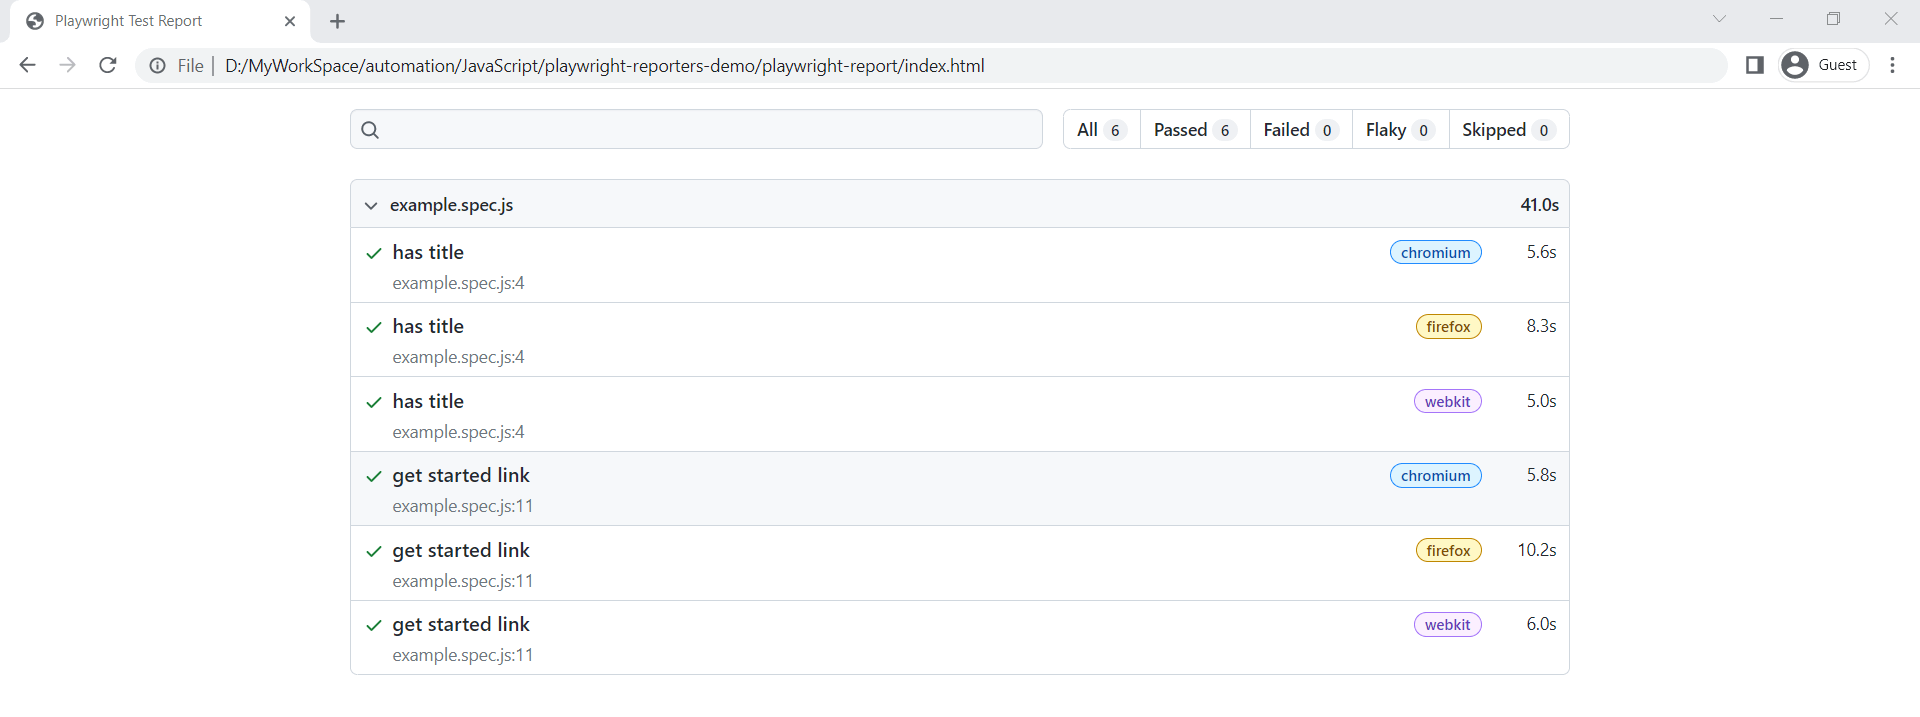
\includegraphics[width=\textwidth]{project/images/playwright-reporting-playwrightreport.png}
    \caption{An example of a Playwright report}
    \label{fig:playwright-report}
\end{figure}

\section{Results and Analysis}

End-to-end testing focused on validating critical user workflows, including account creation, login, and payment processing. Cross-browser tests conducted via BrowserStack revealed rendering inconsistencies in Safari, which were resolved through CSS optimizations. Lighthouse metrics showed significant improvements in performance, with page load times reduced by 30\% on average.
\subsection{Test Coverage}

The QA team tested all critical user journeys, such as account creation, login, and payment processing, ensuring these workflows functioned without issues across various devices and browsers.

\subsection{Cross-Browser Testing}

The QA team performed cross-browser testing to validate the application on different browsers, including Chrome and Firefox. The team identified browser-specific issues and reported them for resolution.

The team used BrowserStack Live to run the tests on Apple's Safari browser on different devices.

\subsection{Performance Considerations}

The QA team monitored the performance of the web application during the E2E testing. The team identified performance issues, such as slow loading times and unresponsive pages, and reported them for resolution.

The team used Lighthouse to measure the performance of the web application and identify opportunities for improvement.

\begin{figure}[H]
    \centering
    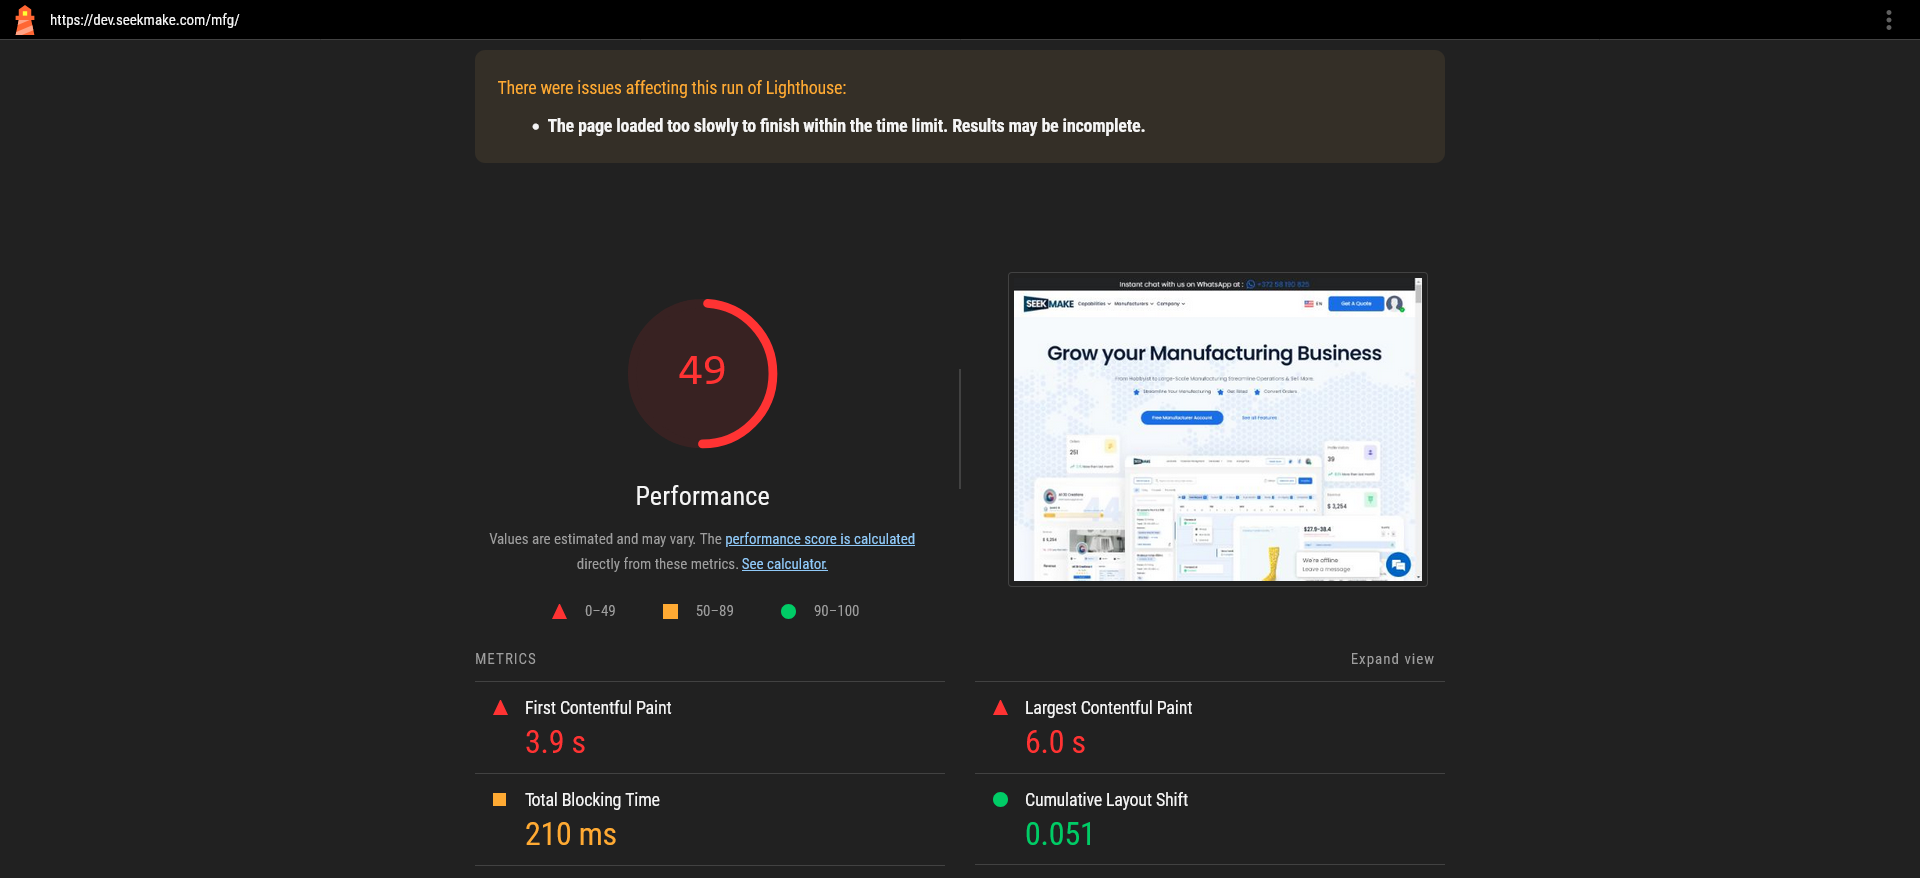
\includegraphics[width=\textwidth]{project/images/lighthouse-report.png}
    \caption{An example of a Lighthouse report}
    \label{fig:lighthouse-report}
\end{figure}

\section{CI/CD Integration}

The QA team integrated the E2E testing framework with the CI/CD pipeline to automate the testing process. The team used GitHub Actions to trigger the test execution on every code change.

\subsection{GitHub Actions Workflow}

The QA team created a GitHub Actions workflow to run the E2E tests on every pull request.

The workflow included steps to install dependencies, build the application, and run the test scripts.

\subsection{Test Automation Pipeline}

The QA team set up a test automation pipeline to automate the E2E testing of the web application.

The pipeline included stages for test execution, test reporting, and test result analysis.

\section{Summary}

The final sprint focused on end-to-end testing of the SeekMake web application. The QA team used Playwright to automate the testing process and validate the functionality, usability, and performance of the application.

The team identified several issues and bugs during the E2E testing, and reported them for resolution.

The team integrated the E2E testing framework with the CI/CD pipeline to automate the testing process. The team used GitHub Actions to trigger the test execution on every code change.
